\chapter{Introduction to Gravitational Lensing}

One of the most amazing results of Einstein's theory of general relativity, regarding the distortion of space time by massive objects is gravitational lensing. The basic principle behind gravitational lensing is that light is distorted when it travels close to the potential well (the distortion of space time) of massive objects (analogous to the effect of optical lenses). Under certain conditions the background objects can be seen in multiple images and ``arcs" surrounding the lensing object, this is known as strong gravitational lensing. 

There are three classes of gravitational lensing:

1. Strong lensing: where there are easily visible distortions such as the formation of Einstein rings, arcs, and multiple images.

2. Weak lensing: where the distortions of background sources are much smaller and can only be detected by analysing large numbers of sources in a statistical way to find coherent distortions of only a few percent

Figure [] is a representation of a lensing system in which a background galaxy is lensed by a cluster of galaxies and produces multiple images as observed from Earth. 

\begin{figure}[H]
\centering
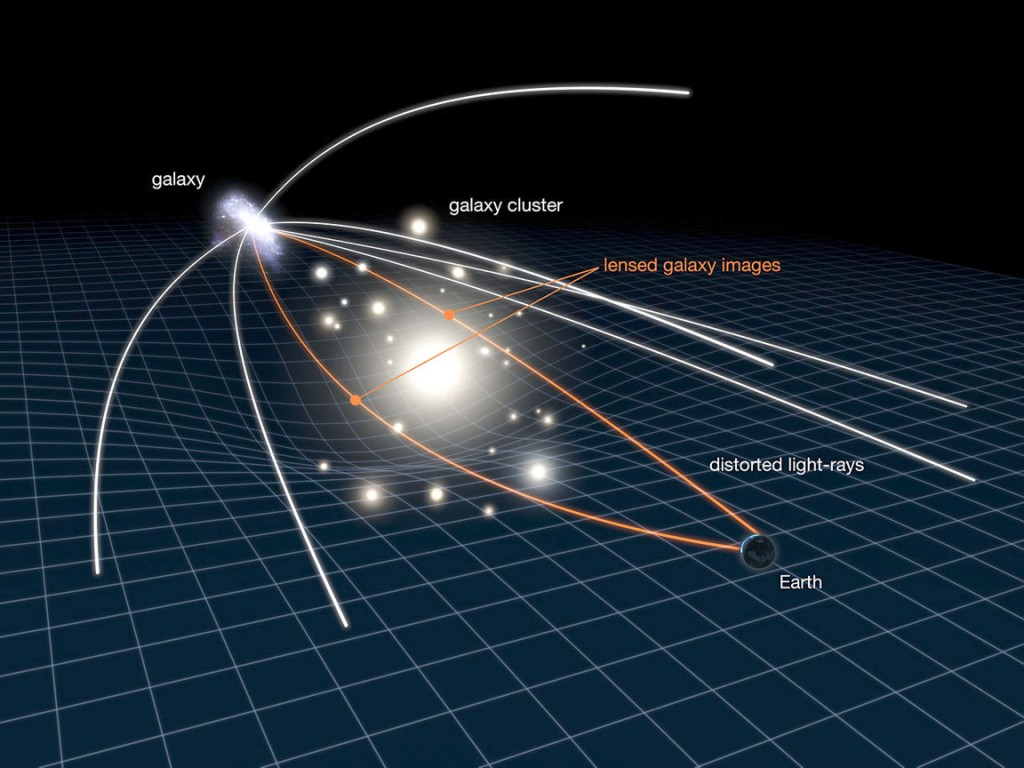
\includegraphics[width=12cm]{images/strong_lensing.jpg}
\caption[Strong Lensing representation]{Nasa?}
\end{figure}

Figure [] is a composite image of a galaxy cluster taken by the HST in which many lensed objects can be seen as distorted shapes and multiple images. 

\begin{figure}[H]
\centering
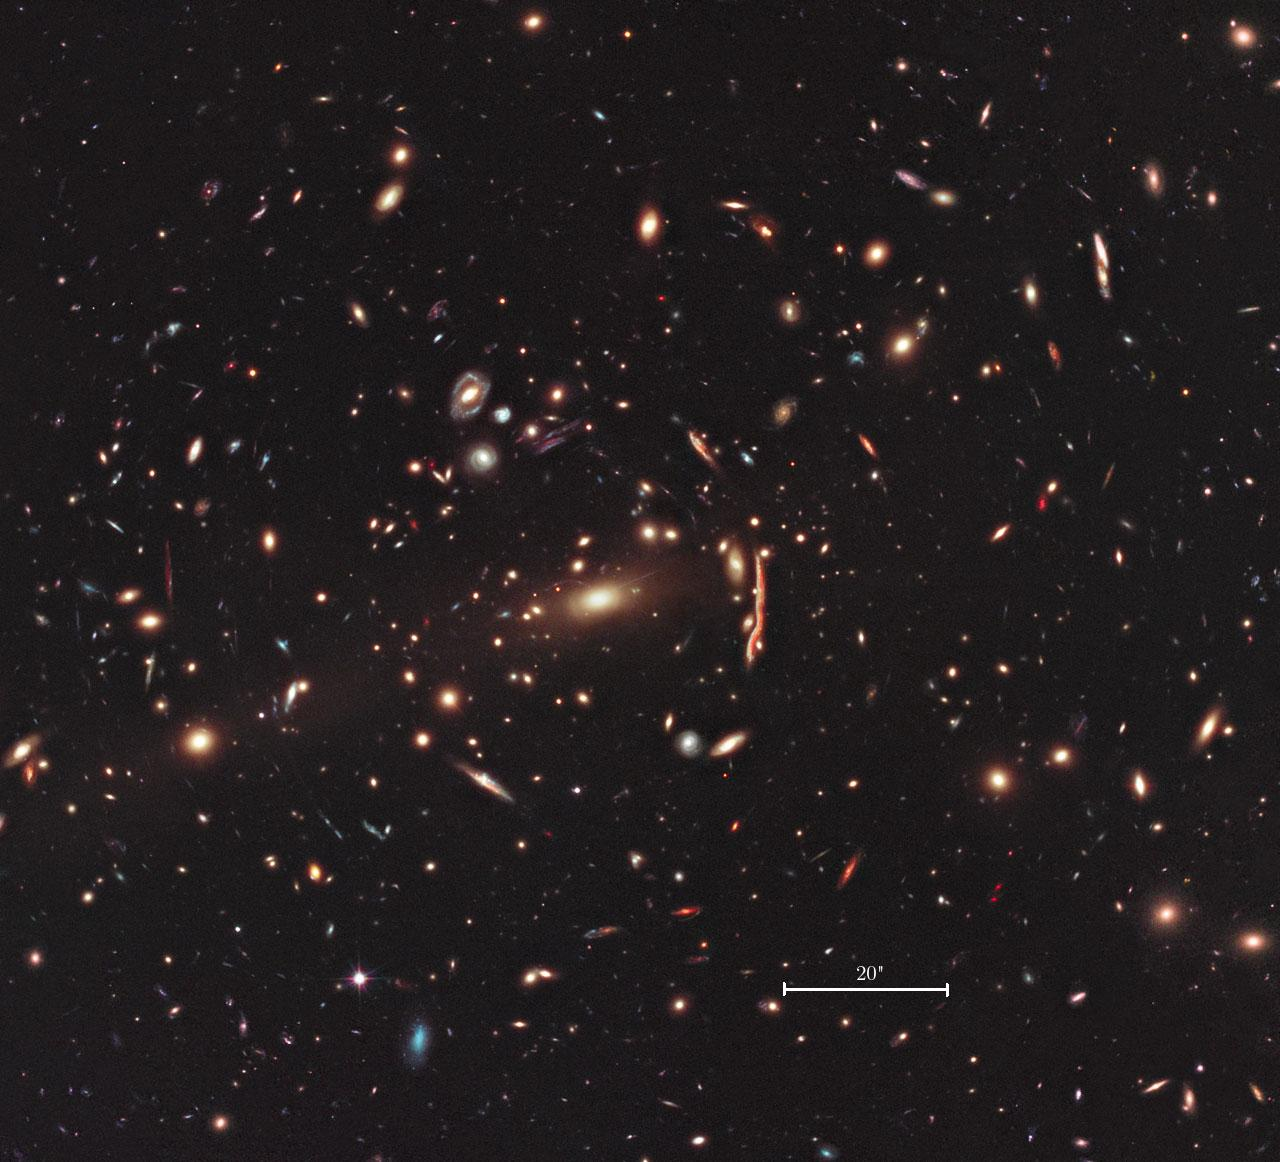
\includegraphics[width=12cm]{images/GC.jpg}
\caption[Galaxy Cluster MACS 1206]{Galaxy Cluster MACS 1206, credits to NASA Hubble Space Telescope}
\end{figure}

Quoted (need to change this): The image of galaxy cluster MACS J1206.2-0847 (or MACS 1206) is part of a broad survey with NASA Hubble Space Telescope. The distorted shapes in the cluster are distant galaxies from which the light is bent by the gravitational pull of an invisible material called dark matter within the cluster of galaxies. This cluster is an early target in a survey that will allow astronomers to construct the most detailed dark matter maps of more galaxy clusters than ever before.These maps are being used to test previous, but surprising, results that suggest that dark matter is more densely packed inside clusters than some models predict. This might mean that galaxy cluster assembly began earlier than commonly thought.

Scientists are planning to observe a total of 25 galaxy clusters under a project called CLASH (Cluster Lensing and Supernova survey with Hubble). One of the first objects observed for the new census is the galaxy cluster MACS J1206.2-0847. This conglomeration of galaxies is one of the most massive structures in the universe, and its gigantic gravitational pull causes stunning gravitational lensing. MACS 1206 lies 4 billion light-years from Earth. In addition to curving of light, gravitational lensing often produces double images of the same galaxy. In the new observation of cluster MACS J1206.2-0847, astronomers counted 47 multiple images of 12 newly identified galaxies.The era when the first clusters formed is not precisely known, but is estimated to be at least 9 billion years ago and possibly as far back as 12 billion years ago. If most of the clusters in the CLASH survey are found to have excessively high accumulations of dark matter in their central cores, then it may yield new clues to the early stages in the origin of structure in the universe.

Galaxies and clusters of galaxies that act as gravitational lenses can be approximated by single isothermal spheres. It is easy to relate an angular scaling parameter $\xi_{E}$, referred to as the Einstein radius, to the mass inside the corresponding light cone. The Einstein radius corresponds to the ring image of a point source aligned exactly on the axis of the lens.

Summary of isothermal sphere:

\begin{equation}
\rho(r)=\frac{\sigma^2}{2\pi Gr^2}
\end{equation}

\begin{equation}
\Sigma(\xi)=\frac{\sigma^2}{2G\xi}
\end{equation}

\begin{equation}
\xi_{E}=4\pi\left(\frac{\sigma}{c}\right)^{2}\frac{D_{ds}}{D_{s}}
\end{equation}

In reality, the density profile and lensing properties of galaxies is a bit more complicated than the assumption of a singular isothermal sphere, so we need to take into account more complex but elaborate profiles such as the NFW (Navarro, Frenk, White, \citeyear{Reference17}).

The NFW density profile is 

\begin{equation}
\rho(r)=\frac{\delta_{c}\rho_{c}}{(r/r_{s})(1+r/r_{s})^{2}}
\end{equation}

where the characteristic over density (dimensionless quantity) is given by:

\begin{equation}
\delta_{c}=\frac{200}{3}\frac{c^{3}}{\ln{(1+c)}-c/(1+c)}
\end{equation}

The mass of an NFW halo contained within a radius of $r_{200}$ is:

\begin{equation}
\text{M}_{200}=\text{M}(r_{200})=\frac{800\pi}{3}\rho_{c}r^{3}_{200}=\frac{800\pi}{3}\frac{\bar{\rho}(z)}{\Omega(z)}r^{3}_{200}
\end{equation}

The concentration parameter $c$ is strongly correlated with Hubble type, c=2.6 separating early from late-type galaxies. Those galaxies with concentration indices $c>2.6$ are early-type galaxies reflecting the fact that the light is more concentrated towards their centres, its formal definition in terms of the virial and characteristic radius is $c=r_{200}/r_{s}$.

Dutton \& Maccio \citeyear{Reference23} (in continuation of previous studies such as Mu\~noz Cuartas et. al. \citeyear{Reference12}), made simulations of halo masses from dwarf galaxies to galaxy clusters and find constraints on the concentration parameter for different redshifts, the relation between the concentration parameter with redshift and virial mass is shown in figure [].

\begin{figure}[H]
\centering
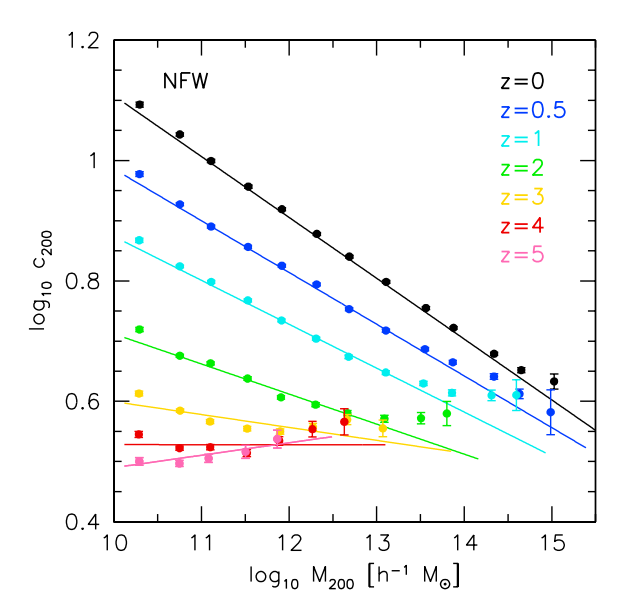
\includegraphics[width=10cm]{images/dutton.png}
\caption[Evolution of the concentration mass relation]{Evolution of the concentration mass relation, by Dutton \& Maccio, \citeyear{Reference23}}
\end{figure}

The surface mass density in the NFW profile is given by:

\begin{equation}
\Sigma_{\text{NFW}}(x) = \left\lbrace
\begin{array}{lll}
\frac{2r_{s}\delta_{c}\rho_{c}}{\left(x^{2}-1\right)}\left[1-\frac{2}{\sqrt{1-x^{2}}}\arctanh\sqrt{\frac{1-x}{1+x}}\right] & (x<1)\\\\
\frac{2r_{s}\delta_{c}\rho_{c}}{3} & (x=1)\\\\
\frac{2r_{s}\delta_{c}\rho_{c}}{\left(x^{2}-1\right)}\left[1-\frac{2}{\sqrt{x^{2}-1}}\arctan\sqrt{\frac{x-1}{1+x}}\right] & (x>1)
\end{array}
\right.
\end{equation} 

so from the critical density:

\begin{equation}
\rho_{c}=\frac{3H^2(z)}{8\pi G}
\end{equation}

$H(z)=H_{0}(1+\Omega z)^{3/2}$

But we are more interested in the enclosed mass which can be done by integrating the surface mass density:

\begin{equation}
\text{M}(R)=\int_{0}^{R}2\pi R\Sigma(R)dR
\end{equation}

The radial dependence on the shear is:

\begin{equation}
\gamma_{\text{NFW}}(x) = \left\lbrace
\begin{array}{lll}
\frac{r_{s}\delta_{c}\rho_{c}}{\Sigma_c}g_{<}(x) & (x<1)\\\\
\frac{r_{s}\delta_{c}\rho_{c}}{\Sigma_c}\left[\frac{10}{3}+4 \ln \left(\frac{1}{2}\right)\right] & (x=1)\\\\
\frac{r_{s}\delta_{c}\rho_{c}}{\Sigma_c}g_{>}(x) & (x>1)
\end{array}
\right.
\end{equation} 

where: 

\begin{equation}
g_{<}(x)=\frac{8 \arctanh \sqrt{\frac{1-x}{1+x}}}{x^{2}\sqrt{1-x^{2}}}+\frac{4}{x^{2}} \ln \left(\frac{x}{2}\right)-\frac{2}{\left(x^{2}-1\right)}+\frac{4 \arctanh \sqrt{\frac{1-x}{1+x}}}{\left(x^{2}-1\right)\left(1-x^{2}\right)^{1/2}}
\end{equation}

\begin{equation}
g_{<}(x)=\frac{8 \arctan \sqrt{\frac{x-1}{1+x}}}{x^{2}\sqrt{x^{2}-1}}+\frac{4}{x^{2}}\ln \left(\frac{x}{2}\right)-\frac{2}{\left(x^{2}-1\right)}+\frac{4 \arctan \sqrt{\frac{x-1}{1+x}}}{\left(x^{2}-1\right){}^{3/2}}
\end{equation} 

and with the critical surface mass density:

\begin{equation}
\Sigma_{c}\equiv\frac{c^{2}}{4\pi G}\frac{D_{s}}{D_{d}D_{ds}}
\end{equation}

these equations come from the paper Wright and Brainerd 1999.

The magnification tensor is:

\begin{equation}
\frac{\partial\beta}{\partial\theta}=\delta_{ij}-\frac{\partial^{2}\psi}{\partial\theta_{i}\partial\theta_{j}}=\left(\begin{array}{cc}
1-\kappa-\gamma_{1} & -\gamma_{2}\\
-\gamma_{2} & 1-\kappa+\gamma_{1}
\end{array}\right)
\end{equation}

The total magnification $\mu$ is given by the determinant of the magnification tensor:

\begin{equation}
\mu = \frac{1}{(1-\kappa)^{2}-\gamma^{2}_{1}-\gamma^{2}_{2}}
\end{equation}


Where $\kappa$ is the convergence that determines the magnification and $\gamma_{1}$ and $\gamma_{2}$ are the shear components that determine the distortion of the background objects.
